%%%%%%%%%%%%%%%%%%%%%%%%%%%%%%%%%%%%%%%%%
% Stylish Article
% LaTeX Template
% Version 2.1 (1/10/15)
%
% This template has been downloaded from:
% http://www.LaTeXTemplates.com
%
% Original author:
% Mathias Legrand (legrand.mathias@gmail.com) 
% With extensive modifications by:
% Vel (vel@latextemplates.com)
%
% License:
% CC BY-NC-SA 3.0 (http://creativecommons.org/licenses/by-nc-sa/3.0/)
%
%%%%%%%%%%%%%%%%%%%%%%%%%%%%%%%%%%%%%%%%%

%----------------------------------------------------------------------------------------
%	PACKAGES AND OTHER DOCUMENT CONFIGURATIONS
%----------------------------------------------------------------------------------------

\documentclass[fleqn,10pt]{SelfArx} % Document font size and equations flushed left

\usepackage[english]{babel} % Specify a different language here - english by default

\usepackage{lipsum} % Required to insert dummy text. To be removed otherwise

\usepackage[defaultfam,light,tabular,lining]{montserrat} %% Option 'defaultfam'
%% only if the base font of the document is to be sans serig
\usepackage[T1]{fontenc}
\renewcommand*\oldstylenums[1]{{\fontfamily{Montserrat-TOsF}\selectfont #1}}

\graphicspath{ {./images/} }

%----------------------------------------------------------------------------------------
%	COLUMNS
%----------------------------------------------------------------------------------------

\setlength{\columnsep}{0.55cm} % Distance between the two columns of text
\setlength{\fboxrule}{0.75pt} % Width of the border around the abstract

%----------------------------------------------------------------------------------------
%	COLORS
%----------------------------------------------------------------------------------------

\definecolor{color1}{RGB}{102, 102, 102} % Color of the article title and sections
%\definecolor{color1}{RGB}{178,34,34} % Color of the article title and sections
%\definecolor{color1}{RGB}{246,64,96} % Color of the article title and sections

%\definecolor{color2}{RGB}{0,20,20} % Color of the boxes behind the abstract and headings
\definecolor{color2}{RGB}{246,64,96}
%----------------------------------------------------------------------------------------
%	HYPERLINKS
%----------------------------------------------------------------------------------------

\usepackage{hyperref} % Required for hyperlinks
\hypersetup{hidelinks,colorlinks,breaklinks=true,urlcolor=color2,citecolor=color1,linkcolor=color1,bookmarksopen=false,pdftitle={Title},pdfauthor={Author}}

%----------------------------------------------------------------------------------------
%	ARTICLE INFORMATION
%----------------------------------------------------------------------------------------

\JournalInfo{
\includegraphics[scale=0.125]{NeoMeetup}} % Journal information
\Archive{ } % Additional notes (e.g. copyright, DOI, review/research article)

\PaperTitle{NeoMeetup: blabla} % Article title

\Authors{Dario Bertazioli\textsuperscript{1}, Fabrizio D'Intinosante\textsuperscript{1}, Massimiliano Perletti\textsuperscript{1}*} % Authors
\affiliation{\textsuperscript{1}\textit{Data Science, Department of Computer Science, University of Milano Bicocca, Milan, Italy}} % Author affiliation
\affiliation{*\textbf{Corresponding author}: m.perletti@campus.unimib.it} % Corresponding author

\Keywords{Meetup --- ADD KEYWORDS--- Keyword3} % Keywords - if you don't want any simply remove all the text between the curly brackets
\newcommand{\keywordname}{Keywords} % Defines the keywords heading name

%----------------------------------------------------------------------------------------
%	ABSTRACT
%----------------------------------------------------------------------------------------

\Abstract{yolo}

%----------------------------------------------------------------------------------------

\begin{document}

\flushbottom % Makes all text pages the same height

\maketitle % Print the title and abstract box

\tableofcontents % Print the contents section

\thispagestyle{empty} % Removes page numbering from the first page

%----------------------------------------------------------------------------------------
%	ARTICLE CONTENTS
%----------------------------------------------------------------------------------------

\section*{Introduction}
{\footnotesize %small for text larger
\textbf{Meetup} è stato creato nel 2002 come piattaforma per mettere in contatto le persone nella vita reale. Fondato e guidato inizialmente da Scott Heiferman e Brendan McGovern, nel 2017 Meetup è stato acquisito da WeWork (ora The We Company). \\
Una volta completata la fase di registrazione, gli utenti possono: \\
\\
- Selezionare i propri interessi: ciò avviene sottoscrivendo dei topic precompilati dall'applicazione in modo da favorire il sistema di raccomandazione. Questi topic spaziano tra i più svariati ambiti, da quello professionale a quello degli hobby, fino ai più comuni, relativi ad eventi sociali. \\
\\
- Iscriversi a gruppi locali: una volta selezionati i topic di interesse il sistema di raccomandazione dell'applicazione suggerisce all'utente una serie di gruppi più o meno locali (a seconda dell'area di interesse selezionata dall'utente) che trattano i topic in oggetto o altri topic ad essi correlati. Ciò permette agli utenti di incontrare persone della propria zona che condividono le stesse passioni. Nel caso in cui tra i topic di interesse per l'utente ce ne siano alcuni che non trovano nessun riscontro in gruppi presenti sul territorio, l'applicazione suggerisce all'utente di creare lui stesso un gruppo con oggetto quel topic, consigliando di mettersi in contatto con altre persone che dimostrano quell'interesse, suggerendole attraverso il sistema di raccomandazione.\\
\\
- Partecipare ad eventi: i gruppi locali, nel corso del tempo, organizzano eventi, incontri, meeting con oggetto i topic dichiarati dai gruppi stessi. Una volta che un gruppo ha organizzato un evento l'utente può visualizzarli sulla propria home e, una volta visionati i dettagli, decidere di comunicare se partecipare oppure no e, nel caso volesse partecipare, se ha intenzione di portare degli ospiti, il tutto in maniera non vincolante. Inoltre, per non restringere troppo la sfera di interessi degli utenti, l'applicazione permette anche di selezionare diversi filtri per la home, tra cui uno apposito per visualizzare eventi organizzati da gruppi di cui non si fa parte o un filtro apposito per visualizzare gruppi di cui l'utente non è già membro e che magari non trattano topic per cui l'utente ha dichiarato interesse, ma che essendo pur sempre gruppi locali, l'utente potrebbe gradire o trovare interessanti.\\
\\
Il focus centrale dell'intero meccanismo dell'applicazione risulta quindi essere quello del "gruppo" visto come realtà associativa e fautore di momenti di aggregazione durante l'intero anno, molto spesso non guidati da una ristretta cerchia di capi ma, anzi, promotore di iniziative da parte dei suoi stessi membri. La varietà di gruppi, a seconda dei topic trattati, spazia tra:
\begin{enumerate}
\item Gruppi di socializzazione, che hanno come obiettivo principale quello di svolgere attività ludiche in compagnia, molto spesso anche promotori di veri e propri eventi di incontro per single.
\item Gruppi professionali, che si pongono l'obiettivo di mettere in contatto persone e professionisti di svariati campi attraverso workshop o presentazioni con il fine di fare crescere gli utenti dal punto di vista professionale.
\item Gruppi creativi, ovvero gruppi di progettazione e più vocati ad hobby ed alla pratica delle più svariate arti. \\
\end{enumerate}
Sintetizzando, quindi, la missione di Meetup è aiutare le persone a crescere e raggiungere i loro obiettivi attraverso connessioni autentiche e reali. Dal network professionale alla birra artigianale passando per workshop di programmazione, le persone usano Meetup per uscire dalla loro comfort zone, incontrare nuove persone, imparare cose nuove, perseguire le loro passioni e trovare sostegno in comunità che le aiutano a crescere.\\
Ad oggi, Meetup è disponibile in 186 Paesi, e conta più di 40 milioni di membri sulla piattaforma, con più di 320 mila gruppi attivi ed una media di 12 mila eventi al giorno.
}
%------------------------------------------------

\section{Goals}
{\footnotesize
Con l'analisi della rete sociale di Meetup e andando a studiare le relazioni che interconnettono le persone attraverso eventi sociali organizzati dai diversi gruppi presenti in tutto il globo, è possibile avere una mappatura più o meno dettagliata degli interessi comuni che portano ad agglomerare un significativo numero di soggetti instaurando relazioni tra di essi. \\
\\
Ricreando questa rete, l'obiettivo del progetto è quello di identificare correlazioni o tracce significative che possono determinare delle buone regole nella creazione di eventi di notevole impatto sociale; una piccola guida '\textbf{How to}' su come dev'essere organizzato un evento di successo. (CONTINUE)%first version incomplete  
}
%------------------------------------------------
\section{Implementation: Architecture}
%FIXME: IMPORTANT: da aggiungere caratteristiche quali tolerance failure et similia un po' ovunque
\subsection{Source}%WebSocket (RSVP) Rest API
Meetup mette a disposizione parte dei dati in suo possesso relativi a membri iscritti alla piattaforma, gruppi creati ed eventi organizzati nella stessa. In particolare, i dati sono forniti in due modalita: 

\paragraph{streaming data:} 
la piattaforma condivide dati in streaming, composti essenzialmente da \textbf{RSVP}.
Le RSVP sono risposte di feedback da parte degli utenti comunicanti agli organizzatori di un evento la loro partecipazione (o la loro non partecipazione, in quanto le risposte possono essere anche negative).
Un esempio di dato del genere è riportato sotto allo scopo di mostrarne la struttura.%FIXME: add fig.
%da fare un format migliore
\begin{itemize}[noitemsep]
\item \textbf{event}:
	\begin{itemize}[noitemsep]
	\item event\_id:	Unique alphanumeric identifier
	\item event\_name: Name of the event
	\item event\_url: URL to the full event page
	\item time: Event time if set in milliseconds since the epoch
	\end{itemize}
\item \textbf{group}:
	\begin{itemize}[noitemsep]
    \item group\_city: Group's home city
    \item group\_country: two-letter code of group's home country
    \item group\_id: Numeric identifier of the group
    \item group\_lat: Latitude of group's approximate location
    \item group\_lon: Longitude of group's approximate location
    \item group\_name: Name of the group
    \item group\_state: two-letter code of group's home state, if in US or CA
    \item group\_topics: Topics associated with this group
			\begin{itemize}[noitemsep]
			\item topic\_name: Longer name
        	\item urlkey: Unique keyword
			\end{itemize}
    \item group\_urlname: Unique portion of group's URL, no slashes
	\end{itemize}
\item guests: Number of guests the member is bringing
\item \textbf{member}: Member who RSVP'd
	\begin{itemize}[noitemsep]
    \item member\_id: Unique numeric id
    \item member\_name: Full name given
    \item other\_services: e.g. {"twitter": {"identifier": "MeetupAPI"}}
    \item photo: Thumbnail URL for member photo if one exists
	\end{itemize}
\item \textbf{mtime}: Last modified time of this RSVP, in milliseconds since the epoch
\item response: "yes" or "no"
\item rsvp\_id: Unique numeric identifier
\item \textbf{venue}: Venue, if public
	\begin{itemize}[noitemsep]
    \item lat: Latitude of the venue
    \item lon: Longitude of the venue
    \item venue\_id: Unique numeric identifier
    \item venue\_name
	\end{itemize}    
\end{itemize}
Tali dati vengono estratti da websocket, sfruttando Nifi (vedasi prossimo paragrafo).
\paragraph{REST api:} Meetup permette anche un accesso piuttosto flessibile al database, esponendo tramite REST API informazioni riguardo a membri, gruppi ed eventi. Abbiamo sfruttato questa possibilità per arricchire i dati acquisiti in streaming: in particolare, abbiamo proceduto all'enrichment delle informazioni sui membri, integrando per ciascun membro:
\begin{itemize}[noitemsep]
\item la localizzazione spaziale, ovvero le coordinate geografiche (lat/lon)
\item i topic in cui l'utente ha dichiarato di essere interessato al momento dell'iscrizione alla piattaforma.
\end{itemize}
\subsection{Nifi}% Producer and blabla
\begin{figure}
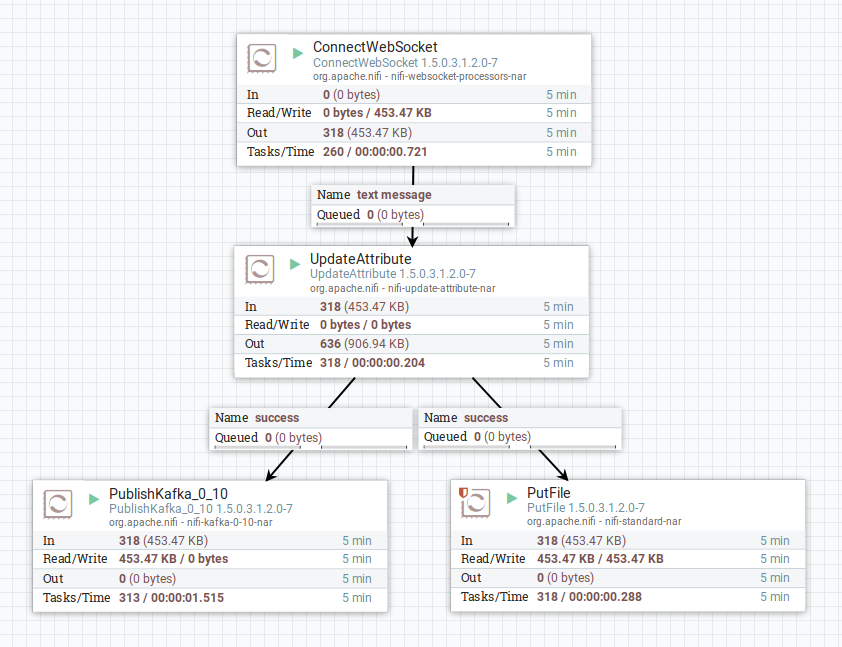
\includegraphics[scale=0.3]{images/nifi_workflow.png}
\caption{\label{nifi_workflow} Il workflow Nifi}
\end{figure}
Per aquisire i dati in streaming dalla piattaforma abbiamo implementato un workflow di Nifi (vedasi fig.~\ref{nifi_workflow}) contenente: 
\begin{itemize}[noitemsep]
\item un nodo per la connessione alla \textbf{WebSocket} (\url{ws://stream.meetup.com/2/rsvps}, tramite un Client Jetty. 
\item un nodo per il parsing iniziale.
\item un nodo \textbf{PutFile}: decidiamo di salvare i dati acquisiti su file system per due motivi principali. Innanzitutto ciò è utile per avere una copia dei dati di backup, qual ora si verificassero problemi (ad esempio, con il corretto setting di \textit{retention time} di Kafka); in secondo luogo, terminato il periodo di acquisizione, per facilitare la copia dei dati su altre virtual machine, in modo da implementare contemporaneamente la stessa pipeline su più macchine, per poter confrontare (quantitativamente, in termini, ad esempio, di quantità di dati importati tempo di esecuzione dei vari scripts etc.) i risultati ottenuti.
\item un nodo PublishKafka, comodo per effettuare l'ingestion dei dati in Kafka (vedasi sezione successiva). %FIXME: forse parentesi non necessaria
\end{itemize} 
I principali vantaggi che Nifi ci ha fornito sono la gestione facilitata della queue, la possibilità di parsing e la facile interfaccia con il Kafka Consumer.
%Inoltre Nifi garantisce %FIXME: aggiungi fault tolerance etc dopo aver fatto check.
\subsection{Kafka} %Lambda Arch. and blabla
Considerata la natura dei dati a nostra disposizione, che ricordiamo consistere flusso di streaming di messaggi (RSVP), abbiamo deciso di fare un'ingestion in Kafka, potendo successivamente esplorare, iterare, e preprocessare le informazioni tramite Python API. 
Abbiamo inoltre modificato i parametri di RetentionTime, in modo tale che Kafka fungesse da primo storage temporaneo, in grado di salvare all'interno di un topic tutti i messaggi acquisiti in real time streaming, per poi poterli processare successivamente senza correre il rischio di perdere qualche informazione.
Come accennato, con l'API di Kafka per Python abbiamo potuto processare i dati, creando diversi csv (link alla repo),%(FIX: non saprei quanto entrare nei dettagli dei vari csv)
 in modo da facilitare e rendere più efficente l'import nel database finale.
%(FIX: eventualmente accenna script per automatizzare)
\subsection{Neo4j}% Storing and querying
Abbiamo scelto di salvare i nostri dati in un database a grafo per via della loro struttura naturale, che ben si presta ad essere schematizzata con nodi principali, proprietà e relazioni che interconnettono tali nodi. Abbiamo provveduto quindi all'import dei dati in Neo4j, sfruttando il linguaggio Cypher e l'ottimizzazione dell'import via csv (accenno alle difficoltà di import precedenti). Per facilitare un'eventuale serializzazione del processo di import, abbiamo creato uno script (Bash) che, una volta creati i csv, consente di automatizzare le varie chiamate alla cypher-shell, dato che il processo di creazione del database risulta piuttosto laborioso ma facilmente standardizzabile (FIX: add link to import.sh).
Aggiungere info quantitative: nodi totali creati, 
\section{Results}

Fabri  $<$3 Meetup xD.
%------------------------------------------------
\phantomsection
\section*{Interesting Challenges}
Circumstances where fabri has sclerated:
\paragraph{Symbolic Links}: Per ovviare a un bug/limite dei nodi getFile/FetchFile che si verifica quando si tenta di fare un'ingestion di una elevata quantità di file in una sola volta, abbiamo escogitato una soluzione creando dei link symbolici, dividendo la creazione in sottocartelle, facendo leggere al nodo GetFile questi link e impostando il nodo in modo che venisse eliminato il link dopo la singola lettura/ingestion. (Va detto ovviamente meglio)
\paragraph{Ottimizzazione script per gestione memoria}: fixme.
\paragraph{Import CSV vs PyNeo}: prestazioni dell'import via csv con Cypher nettamente superiori a quelle ottenute tramite PyNeo (Python API di Neo4j). (aggiungi esempio e amplia)
\paragraph{Scalability}: accenno allo streaming di dicembre, e cenni di scalabilità dato il raddoppio della mole di dati gestiti.

\section*{Acknowledgments} % The \section*{} command stops section numbering

\addcontentsline{toc}{section}{Acknowledgments} % Adds this section to the table of contents

So long and thanks for all the fish.

%----------------------------------------------------------------------------------------
%	REFERENCE LIST
%----------------------------------------------------------------------------------------
\phantomsection
\bibliographystyle{unsrt}
\bibliography{sample}

%----------------------------------------------------------------------------------------

\end{document}